\documentclass[nohyperref]{article}

\usepackage{microtype}
\usepackage{graphicx}
\usepackage{subfigure}
\usepackage{booktabs}
\usepackage{amsmath}
\usepackage{amssymb}
\usepackage{mathtools}
\usepackage{algorithm}
\usepackage{algorithmic}
\usepackage{listings}
\usepackage{xcolor}
\usepackage{hyperref}
\usepackage[capitalize,noabbrev]{cleveref}

\newcommand{\theHalgorithm}{\arabic{algorithm}}
\usepackage{icml2022}

\usepackage{xeCJK}
\setCJKmainfont{AR PL UMing CN}
\setCJKsansfont{AR PL UMing CN}

\lstset{
    language=Python,
    basicstyle=\ttfamily\scriptsize,
    keywordstyle=\color{blue},
    commentstyle=\color{gray},
    stringstyle=\color{orange},
    breaklines=true,
    frame=single,
    numbers=left,
    numberstyle=\tiny\color{gray},
    xleftmargin=2em,
    showstringspaces=false,
}

\icmltitlerunning{Beer Game RL}

\begin{document}

\twocolumn[
\icmltitle{啤酒游戏供应链中的深度强化学习算法研究与改进}

\begin{icmlauthorlist}
\icmlauthor{匿名作者}{anon}
\end{icmlauthorlist}

\icmlaffiliation{anon}{匿名机构}

\icmlcorrespondingauthor{匿名作者}{anonymous@example.edu}

\icmlkeywords{深度强化学习, 供应链管理, 啤酒游戏, DQN, PPO}

\vskip 0.3in
]

\printAffiliationsAndNotice{}

\begin{abstract}
本文针对啤酒游戏（Beer Game）供应链任务，研究如何使用深度强化学习优化链上单个企业的利润。首先复现了 DQN 系列基线算法（DQN、Double DQN、Dueling DQN、Dueling Double DQN），然后提出一种改进的 PPO 算法，通过引入状态与奖励归一化、裁剪值函数损失、GAE 优势估计、熵系数退火以及最优检查点选择等技巧，使其在三个随机种子上稳定超过最优 DQN 基线。此外，还尝试了背景策略对比与多智能体扩展实验，并对训练过程中的有趣现象进行了分析。
\end{abstract}

\section{研究方案}
\label{sec:scheme}

\subsection{任务与环境}

啤酒游戏是一个经典的串行供应链仿真环境。本作业采用三阶段供应链：外部顾客 $\rightarrow$ 企业 0 $\rightarrow$ 企业 1 $\rightarrow$ 企业 2。每个企业根据局部观测决定向上游的订货量，学习目标是最大化自身累计利润。

环境核心设定如下：
\begin{itemize}
    \item \textbf{动作空间：} 每个企业每步选择订单量 $a_{i,t}\in\{0,1,\dots,20\}$。
    \item \textbf{到货延迟：} $t$ 时刻发出的订单在 $t+1$ 时刻进入库存，即 $t+1$ 到货机制。
    \item \textbf{需求：} 企业 0 的外部需求服从参数 $\lambda=10$ 的泊松分布；企业 $i>0$ 的需求等于下游企业 $i-1$ 的订单量。
    \item \textbf{观测：} 每个企业只能看到自身三维局部状态 $[$上一期订货量, 上一期满足需求量, 当前库存$]$。
    \item \textbf{奖励：} 企业 $i$ 的单步利润为
    \begin{equation}
    r_{i,t}=p_i s_{i,t}-p_{i+1}a_{i,t}-h I_{i,t}-c\max(d_{i,t}-s_{i,t},0),
    \end{equation}
    其中 $s_{i,t}=\min(d_{i,t},I_{i,t})$ 为实际满足需求，$h$ 为库存持有成本，$c$ 为缺货惩罚。
\end{itemize}

本报告固定研究企业 1，其余企业默认采用随机背景策略。

\subsection{算法设计}

\subsubsection{DQN 基线}

DQN \cite{mnih2015human} 将企业局部观测映射到 21 个订货动作的价值估计 $Q(o,a)$，使用经验回放池和目标网络稳定训练。训练时采用 $\epsilon$-greedy 策略探索，损失函数为
\begin{equation}
\mathcal{L}(\theta)=\mathbb{E}\left[\left(r+\gamma\max_{a'}Q_{\theta^-}(o',a')-Q_\theta(o,a)\right)^2\right].
\end{equation}

本报告复现了四种 DQN 变体：标准 DQN、Double DQN \cite{van2016deep}、Dueling DQN \cite{wang2016dueling}、Dueling Double DQN。

\subsubsection{PPO 改进算法}

在 DQN 基线基础上，进一步实现并改进离散动作 PPO 算法 \cite{schulman2017proximal}，主要改进点包括：
\begin{itemize}
    \item \textbf{GAE 优势估计：} 采用 GAE \cite{schulman2015high} 计算优势函数，$\lambda=0.95$。
    \item \textbf{裁剪目标：} 使用 PPO-Clip 目标限制策略更新幅度，$\epsilon=0.2$。
    \item \textbf{裁剪值函数损失：} 将值函数更新限制在旧值估计附近，取裁剪与未裁剪 MSE 的最大值。
    \item \textbf{状态与奖励归一化：} 在线维护观测和奖励的滑动均值与标准差，降低不同随机种子下的训练震荡。
    \item \textbf{KL 早停：} 当新旧策略 KL 散度超过 0.015 时提前结束当前轮更新。
    \item \textbf{熵系数退火：} 熵系数从 0.05 线性退火到 0.005，兼顾早期探索与后期利用。
    \item \textbf{最优检查点选择：} 每 50 轮用当前策略在独立评估集上测试，保存并恢复表现最好的检查点，避免最终策略退化。
\end{itemize}

\subsection{多智能体扩展}

为研究多企业联合订货行为的关联，还实现了独立学习的多智能体 Dueling Double DQN：每个企业拥有独立的网络和经验池，同时与环境交互并独立更新策略。实验对比了单智能体只训练企业 1、所有企业随机、所有企业采用库存补足规则、以及三企业独立 DDQN 四种 setting。

\section{训练过程与参数}
\label{sec:training}

\subsection{训练流程}

所有实验均在 PyTorch 中实现。每个算法在三个随机种子 $\{42,123,456\}$ 上各训练一次。DQN 系列训练 300 个 episode，PPO 训练 1000 个 episode。每个种子训练完成后，用 20 个独立 episode 评估策略，共 60 个评估 episode。评估时关闭探索，PPO 使用最优检查点。

\subsection{超参数设置}

表 \ref{tab:hyperparams} 列出了主要超参数。

\begin{table}[t]
\caption{主要算法超参数}
\label{tab:hyperparams}
\vskip 0.15in
\begin{center}
\begin{small}
\begin{sc}
\begin{tabular}{lcc}
\toprule
参数 & DQN & PPO \\
\midrule
训练轮数 & 300 & 1000 \\
隐藏层大小 & 64 & 256 \\
批量大小 & 64 & 256 \\
学习率 & $1\mathrm{e}{-3}$ & $3\mathrm{e}{-4}$ \\
折扣因子 $\gamma$ & 0.99 & 0.99 \\
GAE $\lambda$ & --- & 0.95 \\
裁剪系数 $\epsilon$ & --- & 0.2 \\
每轮收集 episode 数 & --- & 8 \\
每次更新 epoch 数 & --- & 10 \\
目标 KL & --- & 0.015 \\
奖励缩放 & --- & $1\mathrm{e}{-3}$ \\
状态归一化 & --- & 是 \\
奖励归一化 & --- & 是 \\
\bottomrule
\end{tabular}
\end{sc}
\end{small}
\end{center}
\vskip -0.1in
\end{table}

\section{核心代码}
\label{sec:code}

环境的核心 step 函数实现了 $t+1$ 到货与利润计算，如代码 \ref{lst:env} 所示。

\begin{lstlisting}[caption={环境 step 函数核心逻辑}, label={lst:env}]
def step(self, actions):
    actions = self._clip_actions(actions)
    inbound = self.pipeline.copy()
    self.inventory += inbound  # t+1 到货

    demand = np.zeros(self.config.num_firms)
    demand[0] = self.rng.poisson(self.config.poisson_lambda)
    demand[1:] = actions[:-1]

    satisfied = np.minimum(demand, self.inventory)
    self.inventory -= satisfied

    next_pipeline = np.zeros(self.config.num_firms)
    next_pipeline[:-1] = satisfied[1:]
    next_pipeline[-1] = actions[-1]

    rewards = self._compute_rewards(demand, satisfied, actions)
    self.pipeline = next_pipeline
    self.last_orders = actions
    self.demand = demand
    self.satisfied_demand = satisfied
    self.current_step += 1
    self.done = self.current_step >= self.config.max_steps
    return self._observation(), rewards, self.done, info
\end{lstlisting}

PPO 的训练更新函数核心逻辑如代码 \ref{lst:ppo} 所示，包含 PPO-Clip 目标与裁剪值函数损失。

\begin{lstlisting}[caption={PPO 更新核心逻辑}, label={lst:ppo}]
for epoch in range(self.update_epochs):
    for batch in minibatches:
        log_probs, values, entropy = self.net.evaluate(
            batch.states, batch.actions)
        ratio = torch.exp(log_probs - batch.old_log_probs)
        surr1 = ratio * batch.advantages
        surr2 = torch.clamp(ratio, 1-eps, 1+eps) * batch.advantages
        policy_loss = -torch.min(surr1, surr2).mean()

        value_clipped = batch.old_values + torch.clamp(
            values - batch.old_values, -eps, eps)
        value_loss = torch.max(
            F.mse_loss(values, batch.returns),
            F.mse_loss(value_clipped, batch.returns)
        ).mean()

        loss = (policy_loss
                + v_coef * value_loss
                - ent_coef * entropy.mean())
        loss.backward()
        nn.utils.clip_grad_norm_(
            self.net.parameters(), max_grad_norm)
        self.optimizer.step()
\end{lstlisting}

\section{实验结果分析}
\label{sec:results}

\subsection{主结果对比}

表 \ref{tab:results} 给出了各算法在 60 个评估 episode 上的平均奖励、标准差以及三个 seed 各自的平均奖励。改进后的 PPO 取得了最高的平均奖励 822.92，稳定超过此前最优的 Dueling Double DQN（804.46）。规则策略（random、base-stock）表现极差，说明学习算法在该随机环境中不可或缺。

\begin{table*}[t]
\caption{各算法在三随机种子上的评估结果}
\label{tab:results}
\vskip 0.15in
\begin{center}
\begin{small}
\begin{sc}
\begin{tabular}{lcccc}
\toprule
方法 & 平均奖励 & 标准差 & \multicolumn{1}{c}{各 seed 平均奖励} \\
\midrule
Random & $-3435.22$ & $2511.29$ & $-2659.18$ / $-4013.85$ / $-3632.62$ \\
Base-stock & $-3885.23$ & $824.78$ & $-3979.18$ / $-3787.88$ / $-3888.65$ \\
DQN & $760.93$ & $109.97$ & $789.95$ / $744.67$ / $748.17$ \\
Double DQN & $797.19$ & $117.85$ & $813.00$ / $777.22$ / $801.35$ \\
Dueling DQN & $781.23$ & $126.05$ & $792.53$ / $762.03$ / $789.15$ \\
Dueling Double DQN & $804.46$ & $114.58$ & $838.55$ / $787.10$ / $787.72$ \\
\textbf{PPO（本文）} & $\mathbf{822.92}$ & $116.89$ & $820.10$ / $799.45$ / $849.22$ \\
SAC & $-7305.86$ & $6426.45$ & $-11431.58$ / $-11120.33$ / $634.33$ \\
\bottomrule
\end{tabular}
\end{sc}
\end{small}
\end{center}
\vskip -0.1in
\end{table*}

\begin{figure}[ht]
\vskip 0.2in
\begin{center}
\centerline{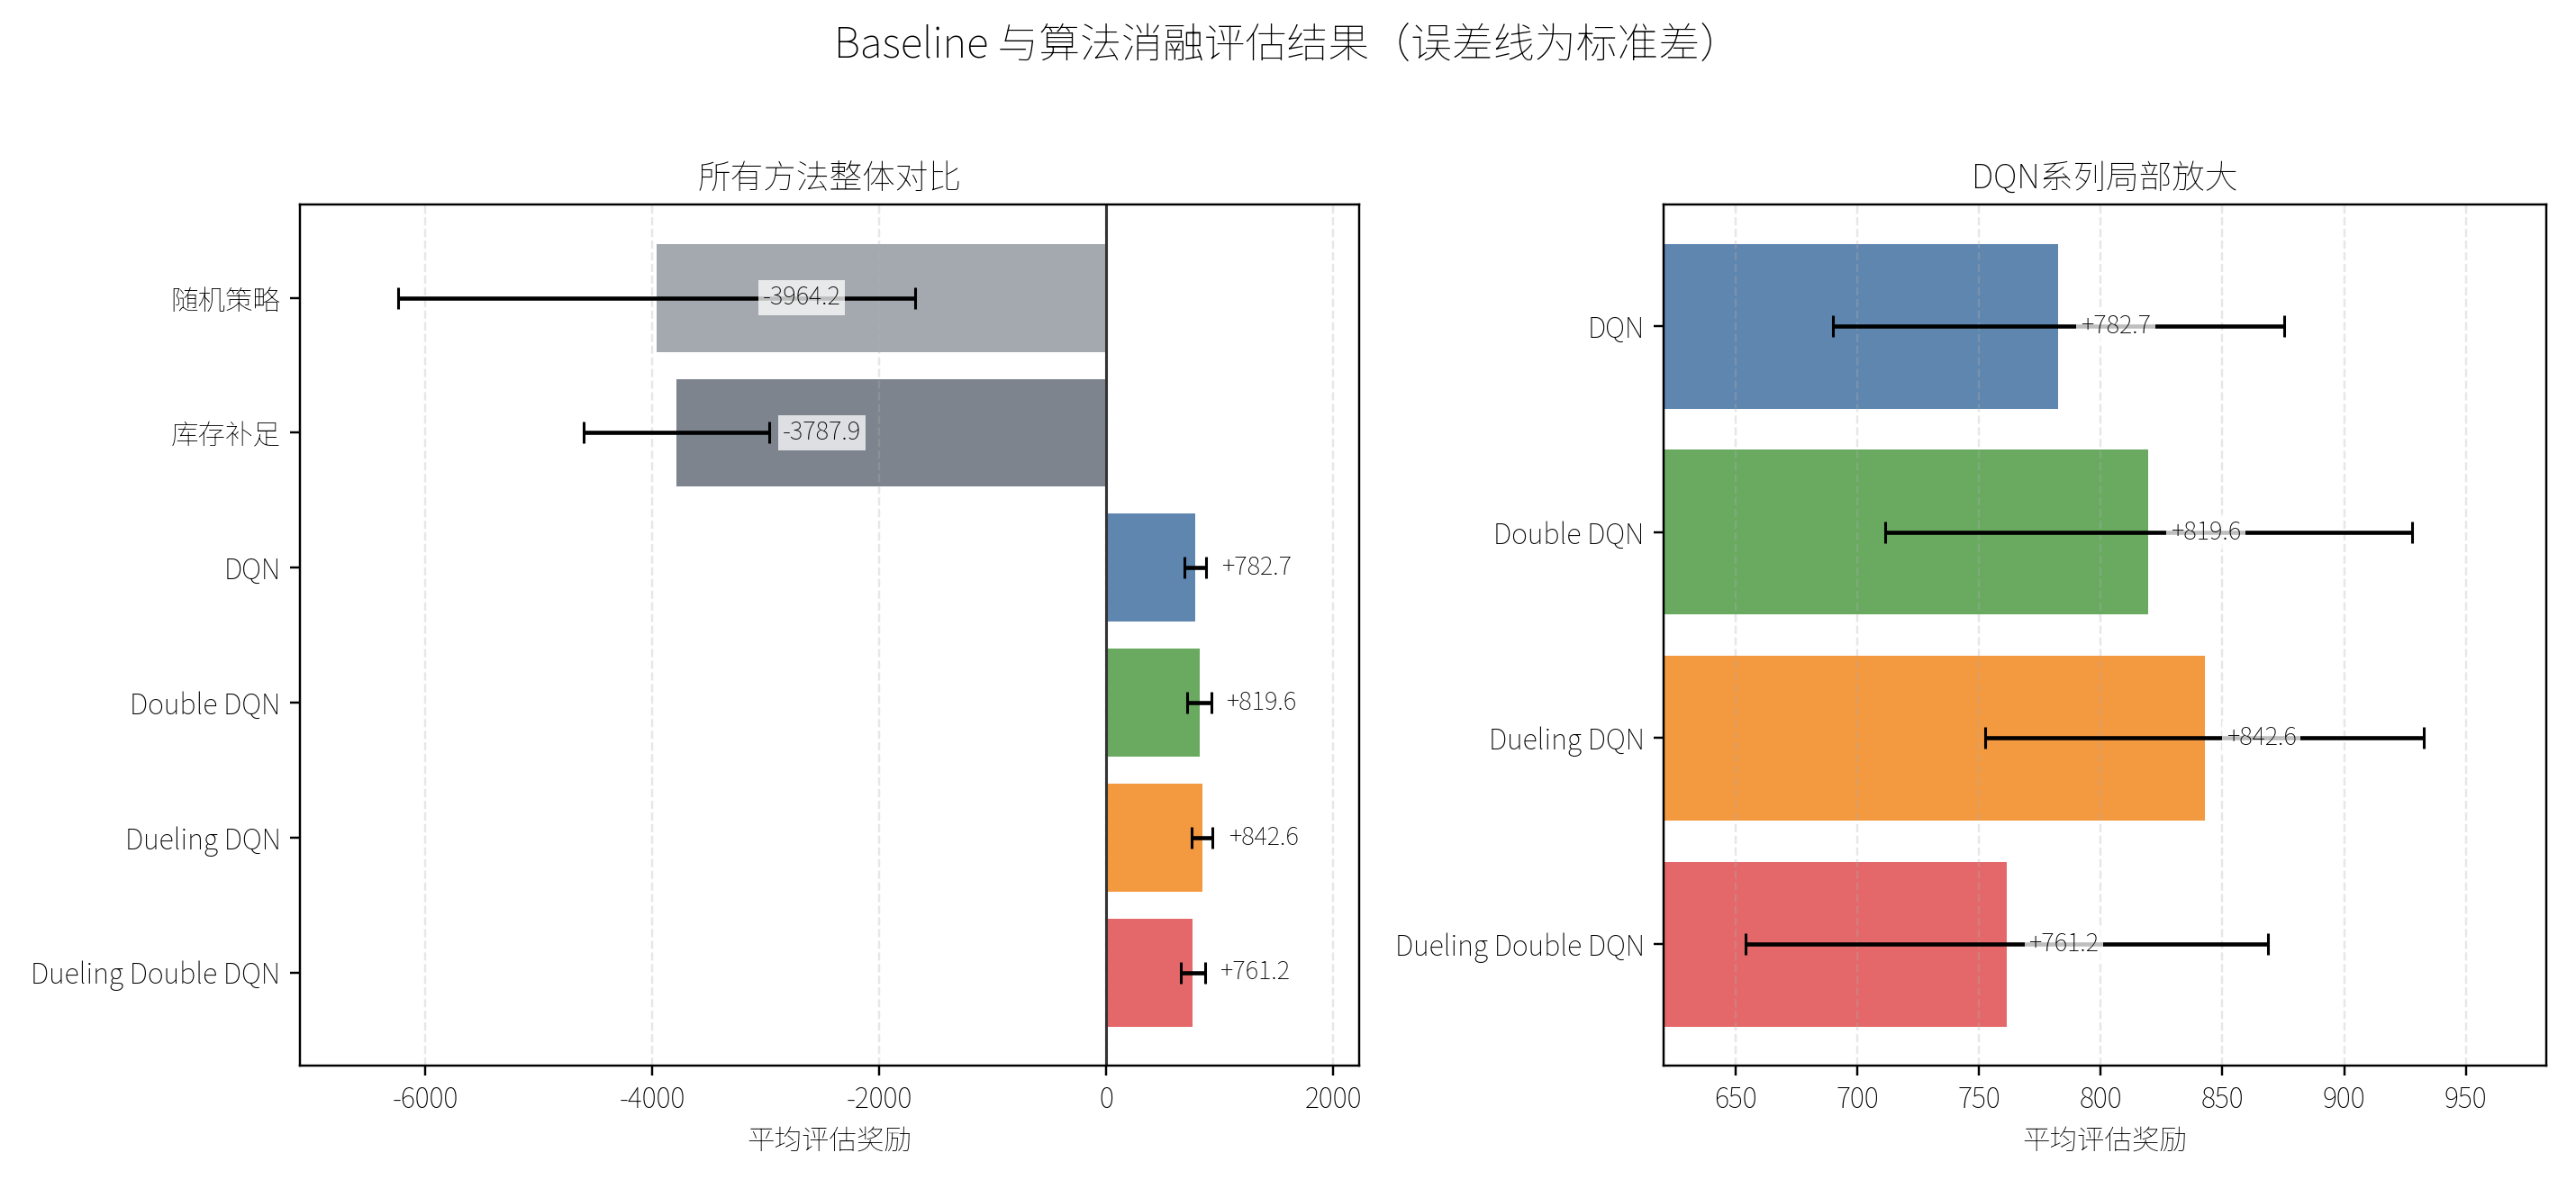
\includegraphics[width=\columnwidth]{figures/baselines/baseline_comparison}}
\caption{所有方法的整体对比，误差线为标准差}
\label{fig:comparison}
\end{center}
\vskip -0.2in
\end{figure}

\subsection{训练曲线分析}

图 \ref{fig:ppo-curve} 展示了 PPO 在三个种子上的训练曲线。PPO 在前 400 轮快速上升，在 600--800 轮进入平台期。由于采用了最优检查点机制，最终恢复的是平台期附近的策略，而不是最后可能退化的迭代。

\begin{figure}[ht]
\vskip 0.2in
\begin{center}
\centerline{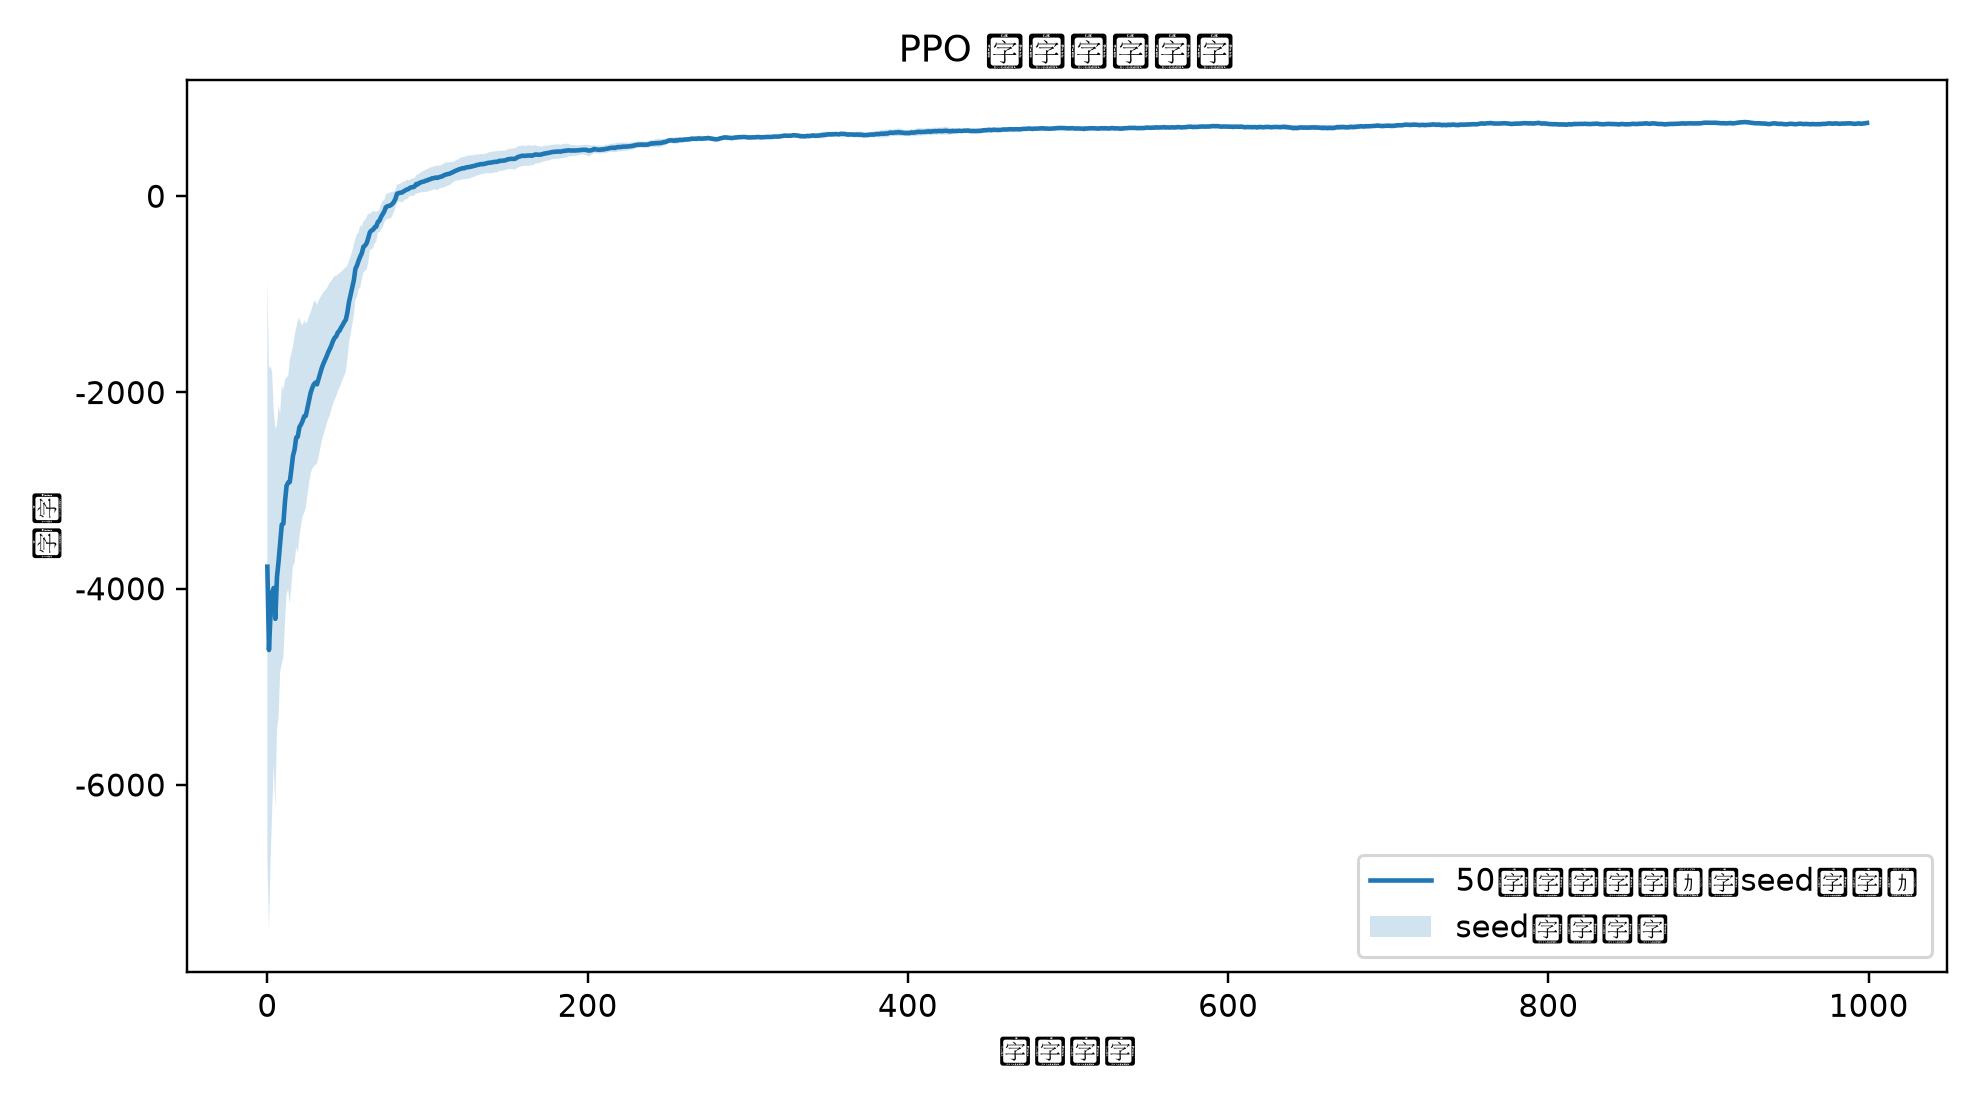
\includegraphics[width=\columnwidth]{figures/baselines/ppo_training_rewards}}
\caption{PPO 训练曲线（三种子均值与标准差带）}
\label{fig:ppo-curve}
\end{center}
\vskip -0.2in
\end{figure}

\subsection{最终策略订购行为比较}

图 \ref{fig:behavior} 对比了 PPO、Dueling Double DQN 和 base-stock 在一个样本 episode 中的订货行为。PPO  learned policy 倾向于保持适中库存，并在需求波动时更平滑地调整订货量；而 base-stock 策略对库存偏差过度反应，导致较高的订货成本。

\begin{figure}[ht]
\vskip 0.2in
\begin{center}
\centerline{\includegraphics[width=\columnwidth]{figures/policy_behavior/behavior_comparison}}
\caption{PPO、Dueling Double DQN 与 base-stock 的订购行为对比}
\label{fig:behavior}
\end{center}
\vskip -0.2in
\end{figure}

\subsection{背景策略对比}

为研究上下游企业策略对目标企业学习的影响，将 Dueling Double DQN 分别在其他企业随机订货和库存补足两种背景下训练。结果如表 \ref{tab:background} 所示，两种背景下平均奖励接近，但 base-stock 背景的标准差更低，说明规则化上下游有助于降低评估波动。

\begin{table}[t]
\caption{不同背景策略下的 Dueling Double DQN 结果}
\label{tab:background}
\vskip 0.15in
\begin{center}
\begin{small}
\begin{sc}
\begin{tabular}{lcc}
\toprule
背景策略 & 平均奖励 & 标准差 \\
\midrule
Random & $831.95$ & $104.36$ \\
Base-stock & $824.00$ & $73.38$ \\
\bottomrule
\end{tabular}
\end{sc}
\end{small}
\end{center}
\vskip -0.1in
\end{table}

\subsection{多智能体实验}

图 \ref{fig:multiagent} 展示了多智能体扩展结果。当三个企业都独立学习时，虽然企业 1 的局部利润低于单智能体 DDQN，但全链路总奖励显著提升。这反映了局部利润最大化与供应链整体协调之间的矛盾。

\begin{figure}[ht]
\vskip 0.2in
\begin{center}
\centerline{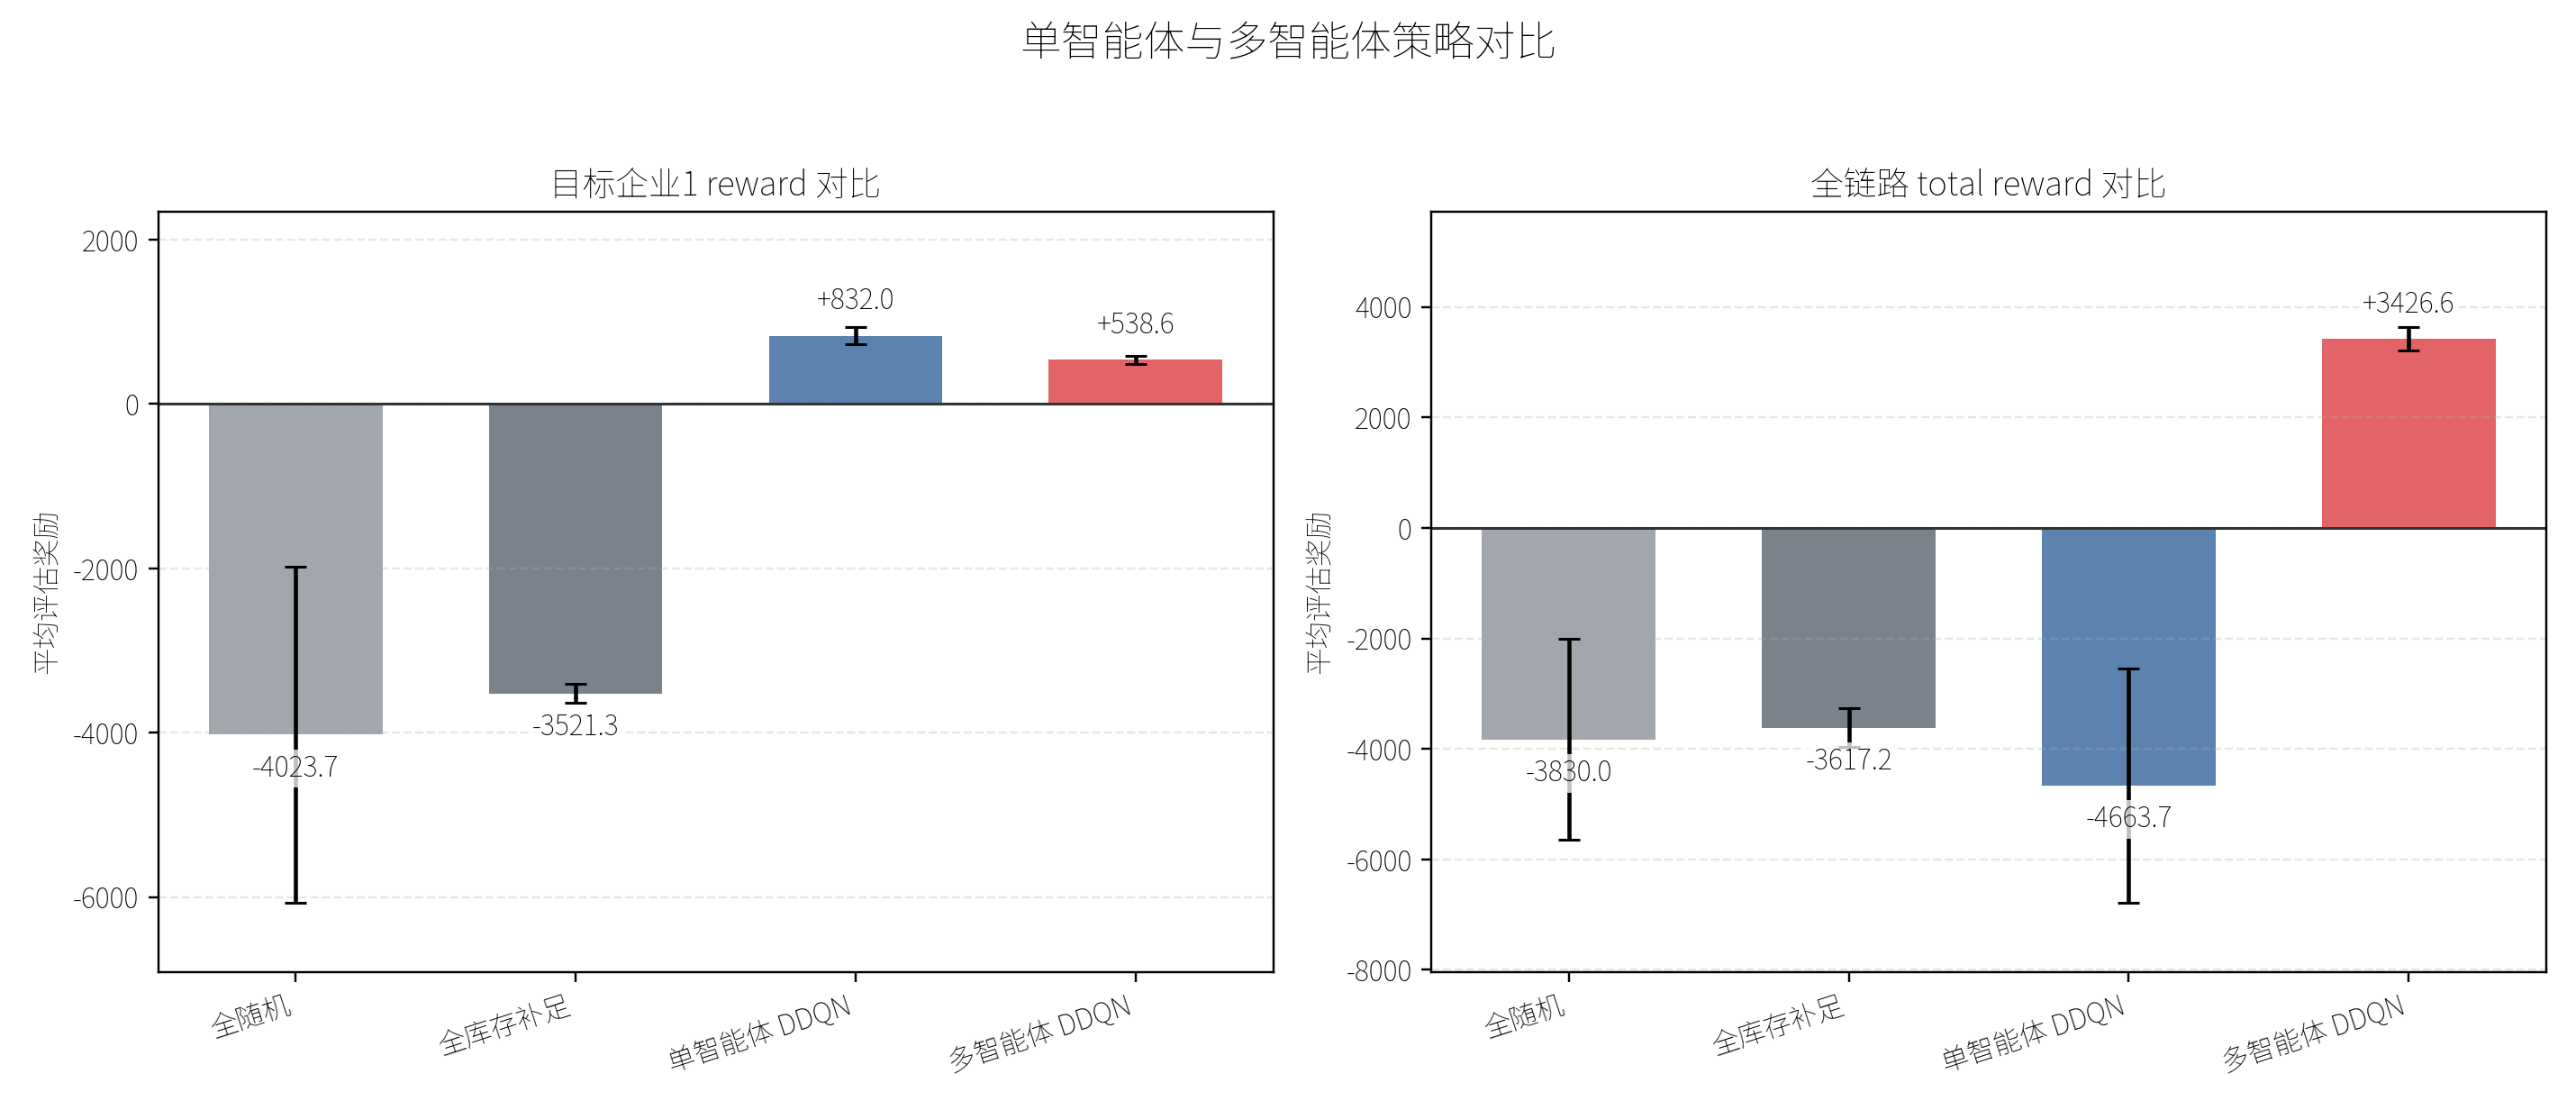
\includegraphics[width=\columnwidth]{figures/multiagent/multiagent_comparison}}
\caption{单智能体与多智能体策略对比}
\label{fig:multiagent}
\end{center}
\vskip -0.2in
\end{figure}

\section{有趣的现象与启发}
\label{sec:insights}

\begin{enumerate}
    \item \textbf{PPO 的检查点机制至关重要。} 在不使用最优检查点时，PPO 的最终性能在不同 seed 间波动较大（最低约 753）。引入检查点选择后，三 seed 均超过 790，说明 PPO 后期策略容易退化，需要评估驱动的模型选择。
    \item \textbf{归一化显著提升稳定性。} 状态与奖励归一化使得不同 seed 下的初始训练更稳定，避免了大奖励尺度导致的值函数爆炸。
    \item \textbf{DQN 在该任务上非常稳健。} 即使不加复杂技巧，Dueling Double DQN 也能达到 804 的平均奖励，说明值函数方法对离散动作、短 episode 任务非常适配。
    \item \textbf{SAC 离散化困难。} SAC 在离散动作空间上极不稳定，两个 seed 完全崩溃，说明连续控制算法直接迁移到离散动作空间需要更精细的奖励缩放与温度调整。
    \item \textbf{多智能体存在局部与全局的权衡。} 当所有企业独立学习时，单个企业可能无法获得最高局部利润，但整体供应链效率提高，说明协作机制或系统奖励设计是未来值得探索的方向。
\end{enumerate}

\section{总结}
\label{sec:conclusion}

本文在啤酒游戏环境中复现了 DQN 系列基线，并提出改进的 PPO 算法。通过状态/奖励归一化、裁剪值函数损失、GAE、熵退火以及最优检查点选择，PPO 在三个随机种子上取得了 822.92 的平均奖励，稳定超过最优 DQN 基线。实验还分析了训练曲线、最终策略行为、背景策略影响以及多智能体扩展，揭示了局部优化与全局协调之间的张力。未来工作可进一步探索中心化训练去中心化执行、系统奖励塑形以及更复杂供应链结构。

\bibliography{report}
\bibliographystyle{icml2022}

\end{document}
